\documentclass{article}
%\setlength{\mathindent}{0pt}
% Package for better handling of figures
\usepackage{graphicx}
% Package for better handling of tables
\usepackage{array}
% Package for better handling of mathematical symbols
\usepackage{mathrsfs}
\usepackage{amsmath}
\usepackage{amssymb}
\usepackage{multirow}
\usepackage{array}
\usepackage{float}


% Title and Author Information
\title{Privacy Preserved Meeting Scheduling}
\author{Group 06}
\date{\today} % You can specify a different date if needed

\begin{document}

% Title Page
\maketitle

% Tentative basic definitions
\section{Tentative basic definitions}

\noindent
Following finite sets are defined:
\begin{itemize}
    \item $\mathcal{D}$: The set of all documents.
    \item $\mathcal{R}$: The set of all roles.
    \item $\mathcal{I}$: The set of all individuals
    \item $\mathcal{L}$: The set of all locations.
    \item $\mathcal{T}$: The set of all time slots.
\end{itemize}

\noindent
Following functions are also defined:
    \[ access: \mathcal{D} \mapsto 2^\mathcal{R} \text{(} 2^\mathcal{R} \text{= power set of } \mathcal{R} \text{)} \] 
    \[ access(d) = \{ r \in \mathcal{R} \mid r \text{ has access to } d \} \] 
    \[ transform: \mathcal{I} \times \mathcal{L} \times \mathcal{T} \mapsto \mathcal{R} \] 
    \[ transform(i, l, t) = r : r \text{ is role of } i \text{ at location } l \text{ at time slot } t \] 
    \[ location: \mathcal{I} \times \mathcal{T} \mapsto \mathcal{L} \] 
    \[ location(i, t)  = l : i \text{ is at } l \text{ at } t \]

\noindent
A meeting M is a 4-tupple,
    \[ M = < D, I, L, t > \]
such that,
    \[ D \subseteq \mathcal{D} \]
    \[ L \subseteq \mathcal{L} \]
    \[ I \subseteq \mathcal{I} \]
    \[ t \in \mathcal{T} \]


% Access Control List
\section{Access Control List}
\noindent
Consider that following finite sets are defined:
\begin{itemize}
    \item $\mathcal{D}$: The set of all documents.
    \item $\mathcal{I}$: The set of all individuals
\end{itemize}
Based on those 2 sets, we define following 2 relationships.
\[ d = \{ d \in \mathcal{D} \mid \text{d is a document} \} \]
\[ access(d) = \{ i \in \mathcal{I} \mid i \text{ has access to } d \} \] \\ 
\noindent
Above relationships mean that $d$ is an element of set $\mathcal{D}$, and that $access(d)$ is the set of individuals ($i$) having access permission to document $d$.\\ 
By 2\textsuperscript{nd} relationship, since any element $i$ of $access(d)$ is also an element of $\mathcal{I}$, we obtain the relationship $access(d) \subseteq \mathcal{I}$. Accordingly, in case all individuals of set $\mathcal{I}$ have access to particular document $d$, $access(d) = \mathcal{I}$.\\
We define any $d$ such that $access(d) = \mathcal{I}$ as a \textbf{public document}. \\ \\

\noindent
Consider that following finite set is also defined:
\begin{itemize}
    \item $\mathcal{G}$: The set of all groups of individuals defined by an entity
\end{itemize}
Based on above all sets, we define following relationship.
\[ access(d) = \{ g \in \mathcal{G} \mid i \text{ has access to } d; i \in g; g \subseteq \mathcal{I} \} \] \\ 
\noindent
Above relationship means that $g$ is an element of set $\mathcal{G}$, and that $access(d)$ is the set of groups ($g$) having access permission to document $d$.\\ 
Since $g$ is a group of individuals ($i$), where $i \in \mathcal{I}$, $g$ is a subset of $\mathcal{I}$. Therefore, we obtain the relationship $g \subseteq \mathcal{I}$.\\
Here we note that, $access(d) = G$ makes $d$ a \textbf{public document}, only if every $i$ exists such that $i \in g$, where $g \in \mathcal{G}$ and $g \subseteq \mathcal{I}$. 
In other words, if there exists any $i$ such that $i \notin g$, then $access(d) = G$ doesn't makes $d$ a \textbf{public document}. \\ \\

% Meeting agenda
\section{Meeting agenda}
\noindent
Agenda of a meeting is the document that defines the set of individuals ($i$) or groups ($g$) required to attend the meeting.
When we consider agenda as document $d$, those individuals ($i$) or groups ($g$) are elements of set $access(d)$.\\ \\
Here, we obviously note that, for agenda, $access(d) \ne \mathcal{I}$. Because, all individuals in set $\mathcal{I}$, are never required to participate in a single meeting.\\ \\
But, there are private meetings and public meetings both. Therefore, for agenda document of any meeting, we define a label as \textbf{privacy label}, stating whether agenda is \textbf{private} or \textbf{public} (i.e. whether meeting is \textbf{private} or \textbf{public}).
\begin{itemize}
    \item If there is at least one onother document in meeting, such that $access(d) \ne \mathcal{I}$, \textbf{privacy label} of agenda must be \textbf{private}.
    \item If every other documents in meeting has $access(d)$ such that $access(d) = \mathcal{I}$, \textbf{privacy label} of agenda can be \textbf{public}.
    \item If agenda is the only document in meeting, \textbf{privacy label} can be used by meeting organizer to define whether agenda document is \textbf{private} or \textbf{public}.
\end{itemize}

\noindent
Following flow chart depicts the process of identifying whether a document is \textbf{private} or \textbf{public}.
\begin{figure}[H]
    \centering
    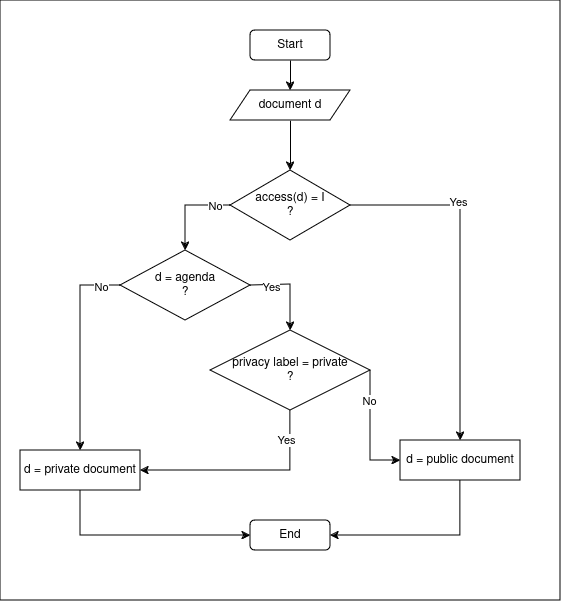
\includegraphics[width=0.7\textwidth]{./image/document_Aug_22.png}
    \caption{Process to identify whether a document is private or public}
    \label{fig:sample}
\end{figure} 

\noindent
In addition to \textbf{privacy label}, meeting agenda should define the \textbf{meeting quorum}, for the meeting. This theme will be discussed later.

% Definition of a meeting
\section{Definition of a meeting}
\noindent
Consider that following finite sets are also defined, other than sets defined above:
\begin{itemize}
    \item $\mathcal{L}$: The set of all locations.
    \item $\mathcal{T}$: The set of all time slots.\\
\end{itemize}
\noindent
\textbf{We assume that every meeting has an agenda associated with it, to define the set of individuals($i$) or groups($g$) required to attend the meeting}. Agenda of a particular meeting $M$ is a document, belonging to set $\mathcal{D}$.\\
When we consider that agenda of meeting $M$ is $d$, for every individual $i$ invited to meeting $M$; $i \in access(d)$. For every group $g$ invited to meeting $M$; $g \in access(d)$. Also consider that, $D$ represents set of documents discussed in $M$, including agenda, such that $D \subseteq \mathcal{D}$. According to our assumption mentioned above, for any meeting $M$; $|D| \geq 1$.\\ \\ 
For conducting a meeting, at least 2 individuals are required. Consider that $I$ represents the set of individuals attending meeting $M$, such that $I \subseteq \mathcal{I}$. Here we note that, for any meeting $M$; $|I| \geq 2$.\\ \\  
Consider set of locations of individuals in $M$ as $L$ (in other words, set of locations of indiduals in set $I$, during meeting time), such that $L \subseteq \mathcal{L}$. Every individual attends meeting from a particular location $l$, such that $l \in L$. We note that if meeting is online or hybrid, $|L| > 1$. If meeting is onsite, $|L| = 1$, since every individual is at same location. Every meeting should be in one mode, out of online, hybrid, onsite modes. $\therefore$ For any meeting $M$; $|L| \geq 1$. \\ \\
Since a \textbf{meeting} is a \textbf{synchrnous} communication, every individual in meeting $M$ should attend the meeting during the same time slot $t$ (Assuming that all individuals are in same time zone).  \\ \\
Based on these definitions, we define meeting M as a 4-tupple,
    \[ M = < D, I, L, t > \]
such that,
    \[ D \subseteq \mathcal{D} \]
    \[ L \subseteq \mathcal{L} \]
    \[ I \subseteq \mathcal{I} \]
    \[ t \in \mathcal{T} \]


% Transformation of individual into role
\section{Transformation of individual into role}
\noindent
Consider that same sets defined above will be used in explanations below, in same notations: \\ \\
\noindent
Consider $i$ and $i'$ as individuals such that $i, i' \in \mathcal{I}$. And consider $d$ as a \textbf{private} document , $l$ as a location and $t$ as a time slot such that $d \in \mathcal{D}$, $l \in \mathcal{L}$ and $t \in \mathcal{T}$.
Further consider that $i \in access(d)$ and $i' \notin access(d)$, for restricting access of document $d$, where $|access(d)| = n$ and $access(d) \ne \mathcal{I}$.\\ \\
\noindent
Assume that at scenario 1, $i$ attends a \textbf{meeting} at location $l$ during time slot $t$ to discuss document $d$, where $i'$ has no access to location $l$ during same time slot $t$. \\
Here we state that privacy of meeting discussing document $d$ was preserved at context $l \times t$ \\ \\ 
\noindent
Now assume that at scenario 2, $i$ attends a \textbf{meeting} at location $l$ during time slot $t$ to discuss document $d$, where $i'$ also has access to location $l$ during same time slot $t$. \\
Here we state that privacy of meeting discussing document $d$ was violated at context $l \times t$, because $n + 1$ individuals including $i'$ have got access to content of document $d$. But actually $|access(d)| = n$ as mentioned above. We observe that $(n + 1) \geq |access(d)| = n$ \\ \\ 
\noindent
When above 2 scenarios are compared, we observe that role of same individual $i$, such that $i \in access(d)$, has experienced a variation. Context of $i$ has changed, depending on location and time. \\ \\
Therefore we define that presence of $i$ at context $l \times t$ transforms $i$ to role $r$.
\[ transform(i, l, t) = r : r \text{ is role of } i \text{ at location } l \text{ at time slot } t \] 
\noindent
If $i \in access(d)$, $i' \notin access(d)$ and $d$ is a \textbf{private} document, $i$ should attend a meeting to discuss $d$ at context $l \times t$, only if $i'$ has no access to $l \times t$. Accordingly, to identify the privacy preserving context for discussing document $d$, combination of i, l, t is required.\\ \\



% Difference between public and private roles
\section{Difference between public and private roles}
When we consider a \textbf{private} document $d$, we can't exactly predict the time, at which $i'$ such that $i' \notin access(d)$, will get access to location $l$. 
Therefore, any location $l$ is defined as a \textbf{private} location, only if access of $i'$ has been strictly restricted, during all potential meeting time slots (represented by set $\mathcal{T}$).\\ \\
Using this definition and above formula, we can show that, $i$ such that $i \in access(d)$ is transformed to $i-private$ role, at a \textbf{private} location. 
Here, location should be defined as a \textbf{private} location, by same entity, that defined the set $access(d)$ for document $d$.

\[ transform(i, l, t) = r \]
\[ transform(i, (private\_location), t) = r \]
\[ transform(i, (private\_location), t) = i-private \] \\

\noindent
On the other hand, any location $l$ is defined as a \textbf{public} location, if access of $i'$ has \textbf{not} been strictly restricted, during any potential meeting time slot (represented by $t$).\\ \\
Using this definition and above formula, we can show that, $i$ such that $i \in access(d)$ is transformed to $i-public$ role, at a \textbf{public} location.
Location should be defined as a \textbf{public} location, by same entity, that defined the set $access(d)$ for document $d$.

\[ transform(i, l, t) = r \]
\[ transform(i, (public\_location), t) = r \]
\[ transform(i, (public\_location), t) = i-public \] \\
\noindent
Based on these derivations, we have identified a constraint relevant to $i$, for discussing $d$ in a privacy preserved meeting.\\ \\
\textbf{Constraint}: When $d$ is a \textbf{private} document, every $i$ such that $i \in access(d)$, that attends a meeting to discuss document $d$, should represent $i-private$ role in the meeting.\\ \\
When $d$ is a \textbf{public} document, any $i$ such that $i \in access(d)$, that attends a meeting to discuss document $d$, is allowed to represent $i-private$ role or $i-public$ role in the meeting.\\ \\

% Variation of role
\section{Variation of role}
\noindent
Now consider a situation where individual $i$ such that $i \in access(d)$ has $x$ number of locations, out of which any one can be selected for attending a meeting to discuss $d$. And assume that $i$ has $y$ number of time slots, out of which any one can be selected for attending the meeting.\\ \\
We can depict the possible variations of $transform(i, l, t)$ function as below, for individual $i$, depending on locations defined by the entity, assuming that $i$ doesn't change location during middle of a time slot.
\begin{table}[H]
    \centering
    \begin{tabular}{|c|c|c|c|c|c|}
    \hline
    $(i)$ & $t_1$ & $t_2$ & $...$ & $t_{y-1}$ & $t_{y}$ \\
    \hline
    $l_1$ & x & x & \  & x & x \\
    \hline
    $l_2$ & x & x & \  & x & x \\
    \hline
    $...$ & \  & \  & \  & \  & \  \\
    \hline
    $l_{x-1}$ & x & x & \  & x & x \\
    \hline
    $l_{x}$ & x & x & \  & x & x \\
    \hline
    \end{tabular}
    \caption{Possibilities in variation of $transform(i,l,t)$ for individual $i$}
    \label{tab:six_columns_six_rows}
\end{table}

\noindent
Note that $l_x$ represents the $x^{th}$ location, while $t_y$ represents the $y^{th}$ time slot. Meanwhile x represents the role of $i$ at the corresponding $l$ and $t$ (based on formula $transform(i, l, t) = r$). According to this representation, we observe that $i$ has $x \times y$ number of possibilities at maximum, to attain the role.\\ \\
Here we emphasize that each x can be categorized as $i-private$ or $i-public$, with respect to the locations defined by entity. According to the constraint identified, if $d$ is a \textbf{private} document, $i$ should attend the meeting only when $r = i-private$. By following this constraint, access of $i'$ such that $i' \notin aceess(d)$, into this meeting can be prevented.\\ \\ 


% Meeting quorum
\section{Meeting quorum}
\noindent
We define \textbf{meeting quorum} as the minimum number of individuals ($i$) required to attend a meeting, such that $i \in access(d)$ and $d$ is the meeting agenda. \\ \\
\textbf{Now consider that agenda is document $\textbf{d}$}, for following description regarding the meeting quorum. In \textit{privacy preserved meeting} context, if a specific \textbf{meeting quorum} isn't defined in the agenda, other than $access(d)$ set, we assume that every $i$ such that $i \in access(d)$, is required for the meeting. Therefore, $|meeting\ quorum| \leq |access(d)|$.\\
Because, it's possible that $|meeting\ quorum| < |access(d)|$, if a specific rule is defined in meeting agenda. \\ \\
Since at least 2 individuals ($i$) are required for any meeting, $2 \leq |meeting\ quorum|$. \\ \\
Accordingly, $2 \leq |meeting\ quorum| \leq |access(d)|$. \\ \\
In real world, since $access(d) \ne \mathcal{I}$, is always true for agenda document, $|access(d)| < |\mathcal{I}|$. Because, all individuals of set $\mathcal{I}$ are never required for a single meeting.\\ \\
$\therefore 2 \leq |meeting\ quorum| \leq |access(d)| < |\mathcal{I}|$ \\ \\
If meeting agenda $d$ defines \textbf{privacy label} as \textbf{private}, then $i'$ such that $i' \notin access(d)$, should be strictly prevented from accessing the meeting, by conducting meeting at a \textbf{private} location, defined by relevant entity.\\ \\
On the other hand, if meeting agenda $d$ defines \textbf{privacy label} as \textbf{public}, then it is \textbf{not} mandatory to prevent access of $i'$ such that $i' \notin access(d)$, for the meeting. Therefore, meeting can be conducted at a \textbf{private} location or \textbf{public} location, based on location definitions of relevant entity.\\ \\

\end{document}

